
\chapter{Real World Example: Stock Exchange Data}
\label{chap:example}
This chapter is about a concrete, real world example. The seminars secondary task was to analyze stock exchange data to find out how fast automated traders respond to published ad~hoc messages. The complete code for this example can be found online at \cite{GitHubAxelPerschmann} and is split into several R scripts:\\

\begin{tabular}[t]{ll}
0\_helloWorld.R & Initial hello world example (\Cref{chap:helloWorld}) \\
1\_dataToHDFS.R & Unzip and transfer stock data into the \ac{HDFS} (\Cref{chap:transferHDFS})\\
2\_parse\_adHocXML.R & Parsing of available adhoc messages (\Cref{chap:adHocMessages})\\
3a\_hadoop\_checkTimeZone.R & Little experiment to verify correct timezone (\Cref{chap:timeZoneCheck})\\
3\_hadoop.R & Defining and running the MapReduce job (\Cref{chap:MapReduceJob}) \\
4\_evaluation.R & Evaluation and plotting of results (\Cref{chap:evaluation})\\
  \end{tabular}

\section{Input Data}
\subsection{Stock exchange data from the Deutsche B\"orse}
The analyzation is based on 166 files (200+ GB) of tick data, obtained from the universities exclusive access to the Deutsche B\"orse. 
Exact to the hundredth of a second they contain millions of transitions, each encoded as follows:

\begin{tabular}[t]{ll}
\texttt{WKN, ISIN} & Instrument identifiers\\
\texttt{INSTRUMENT\_NAME} & Instrument name\\
\texttt{TIMESTAMP, HSEC} & Exact timestamp\\
\texttt{PRICE} & Current price\\
\texttt{UNITS} & Number of units\\
\texttt{BID\_ASK\_FLAG} & BID or ASK\\
  \end{tabular}\\
  
An excerpt from one of the files is shown in \Cref{lst:tickData}.

\begin{lstlisting}[breaklines=true, caption=Excerpt from monthly\_bba\_aa\_20090331.csv., escapechar=|, label={lst:tickData}]
                                                                                   BID_ASK
WKN   ;ISIN        ;INSTRUMENT_NAME          ;TIMESTAMP          ;HSEC;PRICE;UNITS;_FLAG
940602;NL0000009538;KON.PHILIPS.ELECT.  EO-20;2009-03-02 12:04:00; 92 ;12.06; 8572;A
843002;DE0008430026;MUENCH.RUECKVERS.VNA O.N.;2009-03-02 12:04:00; 94 ;92.34;   46;A
840400;DE0008404005;ALLIANZ SE VNA O.N.      ;2009-03-02 12:04:00; 94 ;50.89;   90;A
LYX0A0;FR0010344986;LYXOR ETF DJ ST. 600 RET.;2009-03-02 12:04:00; 94 ;18.29;10000;B
\end{lstlisting}
\label{chap:timeZoneCheck}
In the early phase of testing the subsequent MapReduce job on only one of these 166 input files (monthly\_bba\_aa\_20090331.csv) very little trade activity could be observed. As the given timestamps do not include a timezone definition a little experiment was performed to exclude the case of a miss interpretation. \emph{3a\_hadoop\_checkTimeZone.R} analyzes how trade activity is distributed in terms of daytime. \Cref{fig:timezone} clearly depicts that there is no offset in between observed trades and the trading hours of Xetra which are between 8.50 a.m. CET and 5.30 p.m. CET~\cite{xetra}.

\begin{figure}[ht!]
\centering
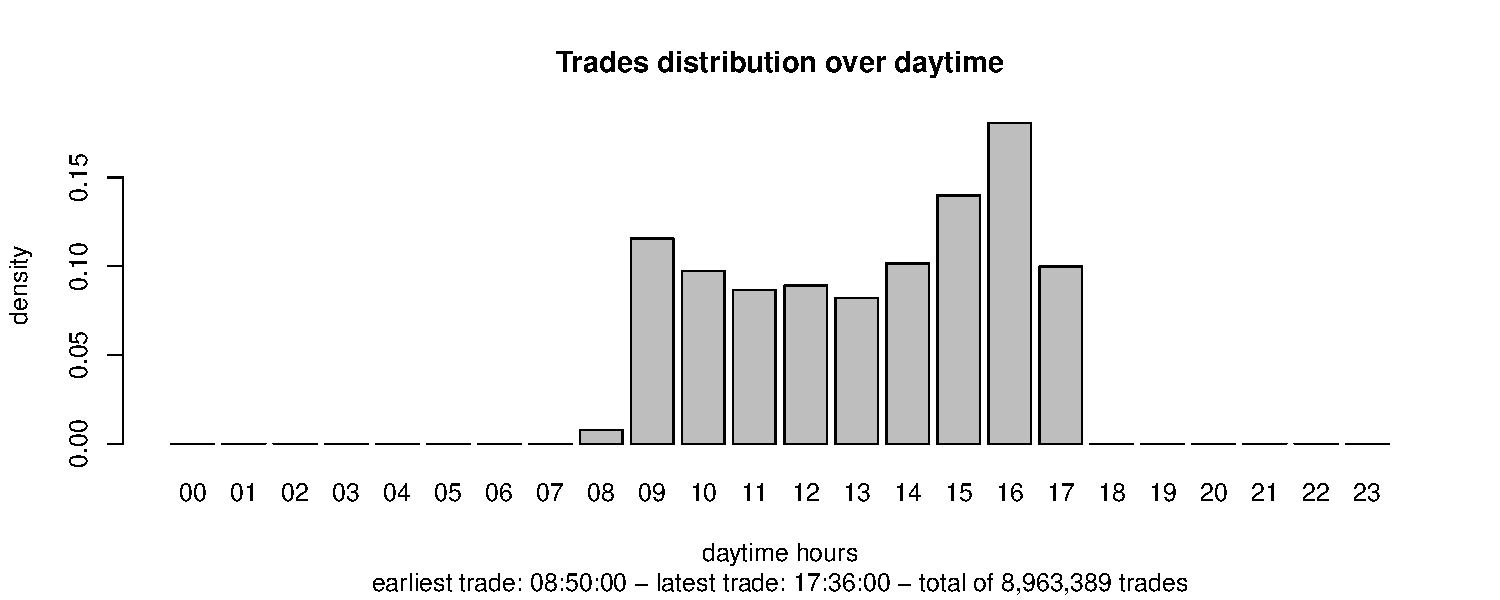
\includegraphics[width=0.7\linewidth]{content/pdf/trade_distribution_new} %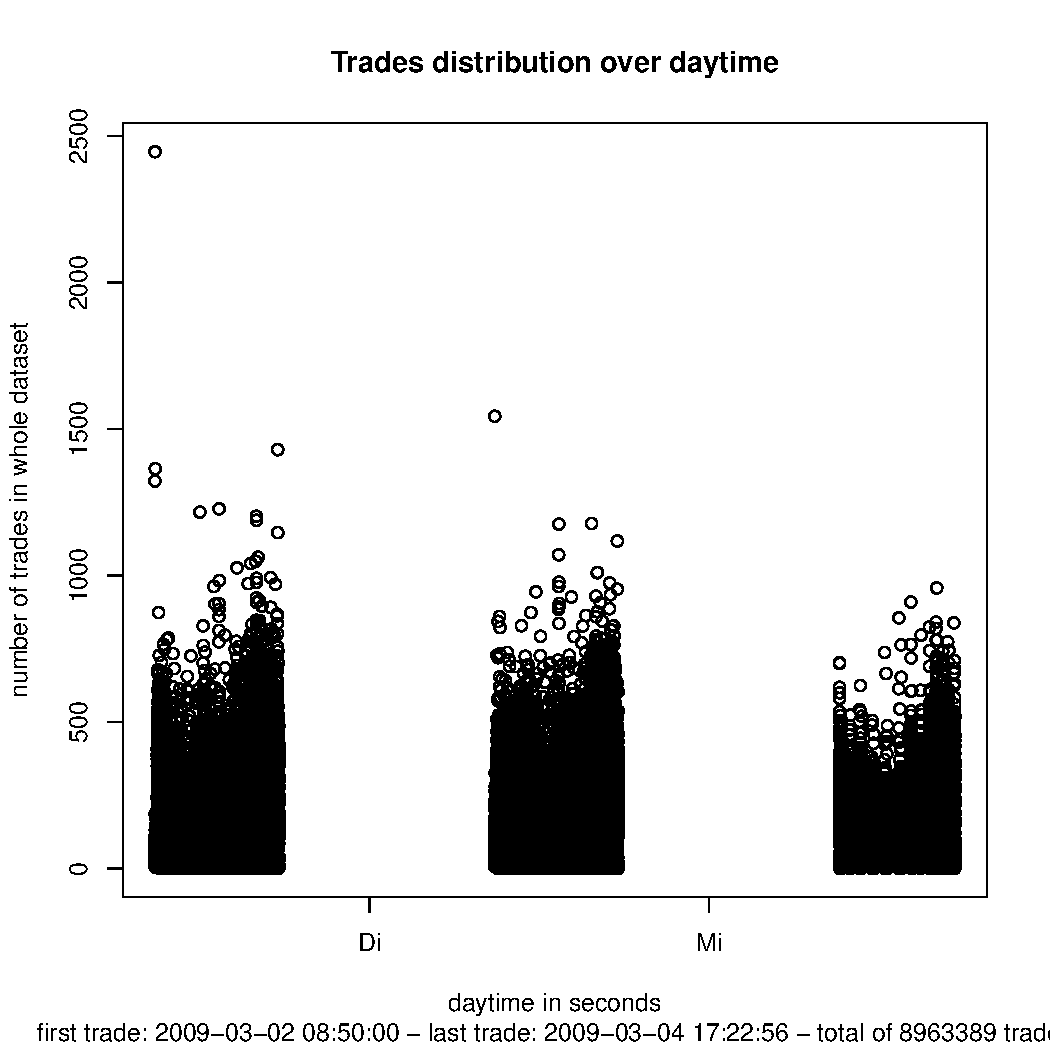
\includegraphics[width=0.35\linewidth]{content/pdf/trade_distribution_date}
\caption{Trade distribution within monthly\_bba\_aa\_20090331.csv.}
\label{fig:timezone}
\end{figure}

\subsection*{Transfer into HDFS}\label{chap:transferHDFS}
All 166 files came as compressed zip files. \Cref{lst:dataToHDFS} shows how these files were unzipped and transferred into the \ac{HDFS}.�\\

As a first step a new directory on the \ac{HDFS} was created using the \lstinline!hdfs.mkdir! command (\Cref{line:mkdir}). Then a for-loop, iterating over all 166 .zip files found in the local directory \lstinline!DeutscheBoerse/!, unzips the contained csv files into a temporary folder \lstinline!DeutscheBoerse/tmp/! and finally transfers the data into the \ac{HDFS} using the \lstinline!hdfs.put! command (\Cref{line:put}). Because the zipped files consume only 260~MB while the unzipped versions take 1.35~GB the latter ones were immediately discarded after they had been transferred to the \ac{HDFS}.

\begin{lstlisting}[breaklines=true, caption=1\_dataToHDFS.R., escapechar=|, label={lst:dataToHDFS}]
Sys.setenv(HADOOP_CMD="/usr/local/hadoop/bin/hadoop")
library(rhdfs)
hdfs.init()

setwd("DeutscheBoerse")
input.names = list.files(path = ".", pattern=".*zip")

# create new directory on HDFS
hdfs.mkdir("/user/isresearch/Data")|\label{line:mkdir}|

# push files to HDFS. Only necessary once!
for (name in input.names) {
  print(name)
  # unzip file and read name of extracted file
  unzip(name, exdir = "tmp/")
  source.name = list.files(path = "tmp")
  
  path.source = paste(getwd(), "/tmp/", source.name, sep="")
  path.dest = paste("/user/isresearch/Data/", source.name, sep="")
  # load to HDFS
  hdfs.put(src=path.source, dest=path.dest)|\label{line:put}|
  
  # do not keep large unzipped file
  unlink(paste(getwd(), "/tmp", sep=""), recursive=TRUE)
}
\end{lstlisting} 

\subsection*{Input format}\label{sec:inputdata}
As we want to process csv files, we have to specify the input format of our mapreduce job, as briefly mentioned in \Cref{sec:rmr2}. In \Cref{lst:inputFormat} we define the csv file separator, the column names and that we do not want strings to be interpreted as factors. Unfortunately \lstinline!make.input.format()! does not come with a parameter like \lstinline!header=TRUE!, such that we have to consider this in our map function where we must discard the headerline.

\begin{lstlisting}[breaklines=true, caption=Input format., escapechar=|, label={lst:inputFormat}]
inputformat <- make.input.format("csv", sep = ";", stringsAsFactors = FALSE,
                              col.names=c("WKN", "ISIN", "INSTRUMENT_NAME", "TIMESTAMP", 
                                           "HSEC", "PRICE", "UNITS", "BID_ASK_FLAG") )
rmr.options(backend="hadoop")
files = hdfs.ls("Data")[,6]         # all filenames in dir /user/isresearch/Data/
files = files[grep(".*csv", files)] # filter for csv files only
\end{lstlisting}


\subsection{Ad~hoc messages}\label{chap:adHocMessages}
An additional collection of seven xml-files ($\approx170$~MB in total) contain individual ad~hoc messages including their respective date and time of publication. The seminars task included the extraction of corresponding (\texttt{TIMESTAMP, ISIN})-pairs using regular expressions. Due to the relatively small size of these xml files this sub task was solved entirely on the local machine and the results stored into a csv file.\\

To make the xml parsing a little complicated, the structure and content of the files vary. In some files the \texttt{ISIN} can directly be read from a field called \lstinline!"isin"!, whereas other files are lacking this field and therefore enforce the use of a regular expression search over the whole message text. Furthermore some messages include only dates and text and do not mention any \texttt{ISIN}. Those messages were discarded and ignored by \emph{2\_parse\_adHocXML.R}. The final version of the regular expression, utilized to extract an \texttt{ISIN} from the raw ad~hoc message text, is shown in \Cref{lst:regEx}.
\begin{lstlisting}[breaklines=true, caption=Regular Expression to extract an ISIN from text., escapechar=$, label={lst:regEx}]
expr = paste("(XS|AD|AE|AF|AG|AI|AL|AM|AO|AQ|AR|AS|AT|AU|AW|AX|AZ|BA|BB|BD|",
               "BE|BF|BG|BH|BI|BJ|BL|BM|BN|BO|BQ|BR|BS|BT|BV|BW|BY|BZ|CA|CC|",
               "CD|CF|CG|CH|CI|CK|CL|CM|CN|CO|CR|CU|CV|CW|CX|CY|CZ|DE|DJ|DK|",
               "DM|DO|DZ|EC|EE|EG|EH|ER|ES|ET|FI|FJ|FK|FM|FO|FR|GA|GB|GD|GE|",
               "GF|GG|GH|GI|GL|GM|GN|GP|GQ|GR|GS|GT|GU|GW|GY|HK|HM|HN|HR|HT|",
               "HU|ID|IE|IL|IM|^IN|IO|IQ|IR|IS|IT|JE|JM|JO|JP|KE|KG|KH|KI|KM|",
               "KN|KP|KR|KW|KY|KZ|LA|LB|LC|LI|LK|LR|LS|LT|LU|LV|LY|MA|MC|MD|",
               "ME|MF|MG|MH|MK|ML|MM|MN|MO|MP|MQ|MR|MS|MT|MU|MV|MW|MX|MY|MZ|",
               "NA|NC|NE|NF|NG|NI|NL|NO|NP|NR|NU|NZ|OM|PA|PE|PF|PG|PH|PK|PL|",
               "PM|PN|PR|PS|PT|PW|PY|QA|RE|RO|RS|RU|RW|SA|SB|SC|SD|SE|SG|SH|",
               "SI|SJ|SK|SL|SM|SN|SO|SR|SS|ST|SV|SX|SY|SZ|TC|TD|TF|TG|TH|TJ|",
               "TK|TL|TM|TN|TO|TR|TT|TV|TW|TZ|UA|UG|UM|US|UY|UZ|VA|VC|VE|VG|",
               "VI|VN|VU|WF|WS|XF|YE|YT|ZA|ZM|ZW)([\\s]?)",
               "(?=.{0,8}[0-9]+)([0-9A-Z]{9}[0-9]?)",
               "(?![0-9]{1})",
               sep="")
  # 2 characters:   country
  # 9 alphanumeric: NSIN
  # 1 number:       optional checksum
\end{lstlisting}

The resulting list of 33\,617 distinct (\texttt{TIMESTAMP, ISIN})-pairs \lstinline!ev! was ordered by \texttt{ISIN} and \texttt{TIMESTAMP} successively and eventually stored into a csv file as shown in \Cref{lst:eventsToCSV}.

\begin{lstlisting}[breaklines=true, caption=Sorting and storage of events.csv., escapechar=$, label={lst:eventsToCSV}]
ev = unique(data.frame(events))

# sort stuff
library(dplyr)
ev = arrange(ev, isin, date)

write.csv(ev, file="events.csv", row.names=FALSE)
\end{lstlisting}

\section{MapReduce Job}\label{chap:MapReduceJob}
Before defining and running the MapReduce job in \Cref{lst:isin.list}, we ensure the previously generated list \lstinline!ev! is available in the global R environment such that our reduce function can access the ad~hoc message dates. We further generate a smaller \lstinline!isin.list! which aggregates all distinct \texttt{ISIN}s contained in \lstinline!ev!, such that our map function can discard data points not belonging to any of these \texttt{ISIN}s.

\begin{lstlisting}[breaklines=true, caption=ev and isin.list are loaded into the global R environment., escapechar=|, label={lst:isin.list}]
# load isin_set
ev = read.csv("events.csv", sep=",", as.is=TRUE, col.names=c("date", "ISIN"))
isin.list = as.character(unique(ev[,2]))
\end{lstlisting}

\subsection{Map() function}\label{sec:mapper}
Multiple, parallel running instances of the Map() function as shown in \Cref{lst:mapFunction} transfer small junks of the whole input into (key, value)-pairs.\\

Each instance receives it's part of the input as value matrix \lstinline!v!, where the different values are accessible by their respective column name (\eg \lstinline!v$PRICE!). The key vector \lstinline!k! is empty, except for the case of chaining multiple MapReduce jobs together.

\begin{lstlisting}[breaklines=true, caption=Map() function., escapechar=|, label={lst:mapFunction}]
map.ticks <- function(k, v) {
  # Skip header lines
  v = v[v$PRICE != "PRICE",]|\label{line:header}|
  v$PRICE = as.double(v$PRICE)|\label{line:double}|
  v = v[v$PRICE != 0.0, ] # erroneous values in data?!|\label{line:erroneous}|
  
  # only extract ISIN's when we have observed an AdHoc msg
  v = cbind(v, useful=v$ISIN %in% isin.list)|\label{line:useful}|
  v = v[v$useful == TRUE,]
  
  keyval(key=paste(v$ISIN, v$BID_ASK_FLAG, sep="_"),
         val=subset(v, select=c("TIMESTAMP", "PRICE")))|\label{line:subset}|
}
\end{lstlisting}

As mentioned in \Cref{sec:inputdata}, we need to filter out the header line. In \Cref{line:header} we discard all rows whose \lstinline!v$PRICE! contains the string \lstinline!"PRICE"! rather than a number. Once the header is gone, we can convert column \lstinline!v$PRICE! from character to double (\Cref{line:double}) and discard erroneous values (\Cref{line:erroneous}). A major reduction of the data is achieved in \Cref{line:useful}, where we check wether a data points \texttt{ISIN} is present in \lstinline!isin.list! (\lstinline!useful=TRUE!) or not (\lstinline!useful=FALSE!). Only useful values will be kept. Finally we define the key as a concatenation of \texttt{ISIN} and \texttt{BID\_ASK\_FLAG} (\eg \lstinline!"DE0007664039_A"!, \lstinline!"DK0010272632_B"!) and the value is further reduced to the columns of interest: \texttt{TIMESTAMP} and \texttt{PRICE}.


\subsection{Reduce() function}\label{sec:reducer}
After the map phase has finished, the ordered (key, value)-pairs are distributed across multiple, parallel running instances of the Reduce() function shown in \Cref{lst:redFunction}.

\begin{lstlisting}[breaklines=true, caption=Reduce() function., escapechar=|, label={lst:redFunction}]
red.ticks <- function(k, v) {
  v$TIMESTAMP = as.POSIXct(v$TIMESTAMP, "%Y-%m-%d %H:%M:%OS", tz="CET")
  v = v[order(v$TIMESTAMP),]
  
  adhocs = ev[ev$ISIN == unlist(strsplit(k, "_"))[1], 1]
  adhocs = as.POSIXct(adhocs, "%Y-%m-%d %H:%M:%OS", tz="CET")
  adhocs = adhocs[!is.na(adhocs)]
  
  # only keep adhoc dates which lay in the interval of available tick data
  adhocs.relevant = adhocs[adhocs > v$TIMESTAMP[1]]|\label{line:adHocFilter}|
  adhocs.relevant = adhocs.relevant[adhocs.relevant < tail(v$TIMESTAMP, n=1)]
  
  if (length(adhocs.relevant) > 0) {
    # compute price deltas for fixed intervals
    l = length(adhocs.relevant)
    offset.seconds = c(0, 1, 5, 10, 30, 60, 60*5, 60*10, 60*60)
    timestamps = matrix(rep(adhocs.relevant,length(offset.seconds)), nrow=l)
    offset = matrix(rep(offset.seconds, l), byrow=TRUE, nrow=l)
    timestamps.future = timestamps + offset
    
    fun = stepfun(v$TIMESTAMP, c(v$PRICE, tail(v$PRICE, n=1)), f=0, right=TRUE)|\label{line:stepFun}|
    
    # collect corresponding PRICE for each TIMESTAMP
    result = c()
    for (i in 1:l) {
      x = fun(timestamps.future[i,])
      result = rbind(result, x)
    }
    colnames(result) = paste("+", offset.seconds, "s", sep="")
    
    # calculate PRICE delta over time
    delta = result / result[,1]
    colnames(delta) = paste("s", offset.seconds, sep="")
    rownames(delta) = make.names(adhocs.relevant, unique=TRUE)
    
    keyval(key=cbind(isin=k, date=as.character(adhocs.relevant)), 
           val=delta)
  }
}\end{lstlisting}
After an initial character to POSIXct\footnote{\url{https://stat.ethz.ch/R-manual/R-devel/library/base/html/DateTimeClasses.html}, accessed: 17-June-2016} conversion and subsequent order-by-time command, we extract all ad~hoc timestamps belonging to the current \texttt{ISIN} from \lstinline!ev!. In \Cref{line:adHocFilter}f. we discard dates of ad~hoc messages that occurred outside the available tick data range. \\

For the remaining adhoc dates we check the stock price 1s, 5s, 10s, 30s, 60s, 5m, 10m and 1h after publication of the particular message and compute the respective deltas in percent. For this purpose, we convert the available stock data points into a step function (\Cref{line:stepFun}). Parameter \lstinline!f=0! disables interpolation between the given x values, such that the functions return value always corresponds to the last price observed before the queried time point.\\

The function finally returns the computed deltas for every applicable (\texttt{ISIN, ad~hoc})-pair.

\subsection{MapReduce job call}
The final call of the MapReduce job is shown \Cref{lst:mapReduceJob}. The variables \lstinline!files! and \lstinline!inputformat! were introduced in chapter \ref{sec:inputdata}, \lstinline!map.ticks! in \Cref{sec:mapper} and \lstinline!red.ticks! in \Cref{sec:reducer}.\\

The job's output will be stored into the \ac{HDFS} as a csv file while the function \lstinline!mapreduce()! returns the associated filepath. To further view or process the data in RStudio \lstinline!from.dfs()! loads the output into the R environment.

\begin{lstlisting}[breaklines=true, caption=Running the MapReduce job., escapechar=|, label={lst:mapReduceJob}]
library(rmr2)
rmr.options(backend="hadoop")

data<- mapreduce(input=files
                 ,input.format=inputformat
                 ,output="user/isresearch/output.csv"
                 ,output.format=make.output.format("csv", sep=";")
                 ,map = map.ticks
                 ,reduce = red.ticks
)
data.df = from.dfs(data, format=make.input.format("csv", sep=";"))
\end{lstlisting}

\section{Evaluation}\label{chap:evaluation}
Once the MapReduce job has finished successfully and the data is loaded into the R environment, we can finally generate some statistics. The examples task was to find out how fast automated traders respond to published ad~hoc messages. The evaluation code is available at \cite{GitHubAxelPerschmann}.\\

\Cref{fig:tradeActivity} shows the ratio of samples where an ad~hoc message was shortly after followed by a price fluctuation. In 58 of 8565 cases (0.7\%) a trade had happened within the first second after the publication, whereas after 1 minute the activity rate was already at 8.6\%. One hour after publication, 29.9\% off all examples where affected by a price fluctuation. The Figure also shows that the majority of these price chances had an upward trend.\\

\begin{figure}[ht!]
\centering
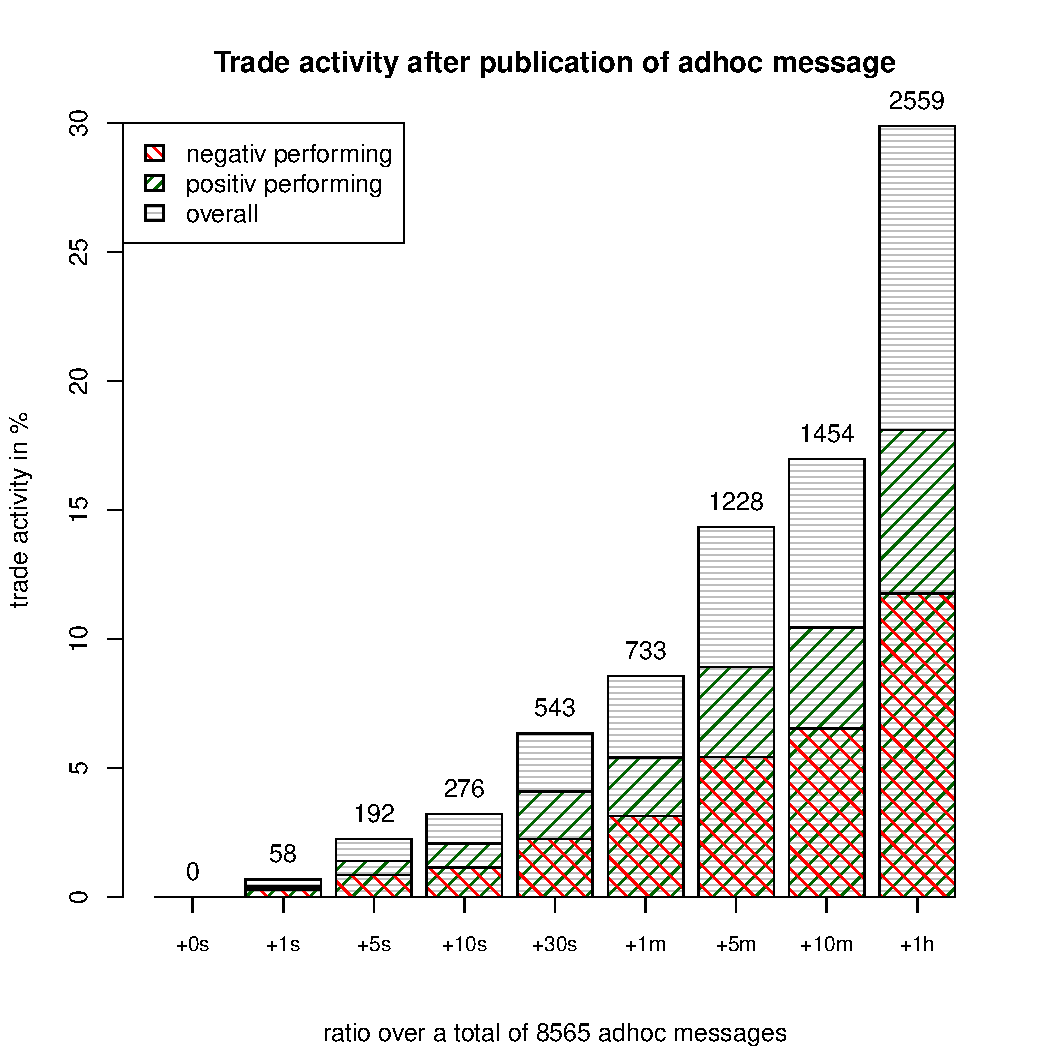
\includegraphics[width=0.70\linewidth]{content/pdf/summary}
\caption{Trade activity after publication of ad~hoc message.}
\label{fig:tradeActivity}
\end{figure}

\Cref{fig:meanPerformance} shows the average stock performance after an ad~hoc message was published. The displayed mean values were calculated from all samples that did show trade activity, \ie the values for '+1s' origin from 58 samples, whereas the values for '+1h' are an aggregation of 2559 values.\\

Nevertheless, since it seems reasonable that within elongating time intervals more trade activity is observed, we can not proof any causality in between the publication of ad~hoc messages and the occurring price fluctuations. In future studies one could analyze preceding points in time as well to compare the trade activity before and after the respective ad~hoc message publication.\\

\begin{figure}[ht!]
\centering
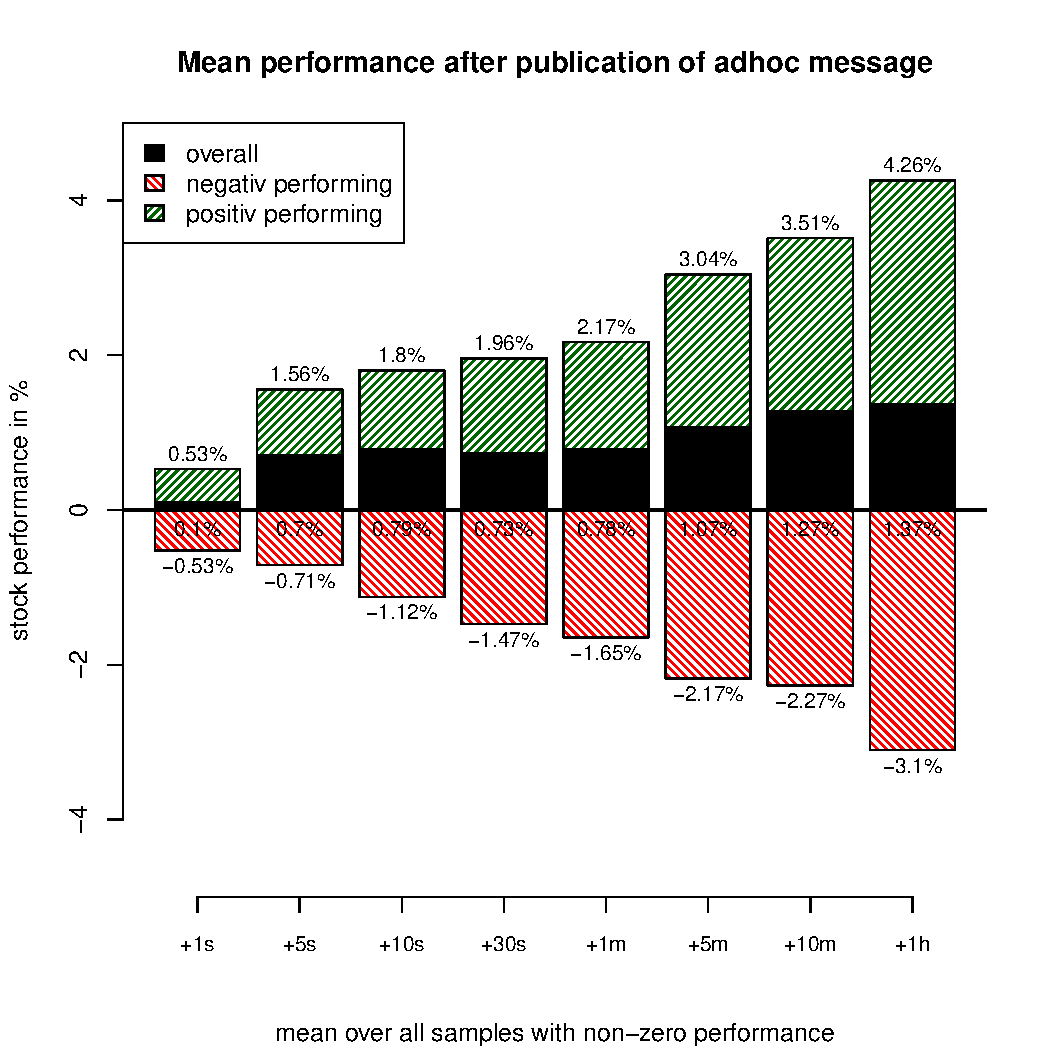
\includegraphics[width=0.70\linewidth]{content/pdf/summary_performance}
\caption{Mean performance after publication of ad~hoc message.}
\label{fig:meanPerformance}
\end{figure}

\chapter{Conclusion}\label{chap:conclusion}
Due to the volume of data, the real world example shown in \Cref{chap:example} would have been a tough job on any single local workstation or students notebook. When analyzing big data, it is a great relief or even an inevitable thing to use a cluster of computer for distributed storage and data processing.\\

Hadoop is a great and powerful cluster framework and R is a highly popular and well-advanced programming language for statisticians. In a world of ever growing data, Hadoop and R make a perfect fit. Both combined, the mightful analytic capabilities of R can be applied to big data.



